% !TeX program = pdflatex
% Informe Técnico - Proyecto Global Integrador AyME
% Archivo base para TeXstudio. Completar los datos marcados con TODO.

\documentclass[10pt,a4paper]{article}

% ---------------------------------------------------------
% PAQUETES
% ---------------------------------------------------------
\usepackage[utf8]{inputenc}
\usepackage[T1]{fontenc}
\usepackage[spanish,es-tabla]{babel}
\usepackage{amsmath,amssymb}
\usepackage{siunitx}
\usepackage{booktabs}
\usepackage{array}
\usepackage{float}
\usepackage{graphicx}
\usepackage{xcolor}
\usepackage{tikz}
\usepackage{fancyhdr}
\usepackage{lastpage}
\usepackage{geometry}
\usepackage{hyperref}
\usepackage{enumitem}

\usetikzlibrary{positioning,arrows.meta}

% ---------------------------------------------------------
% CONFIGURACIÓN GENERAL
% ---------------------------------------------------------
\geometry{
    a4paper,
    left=2.0cm,
    right=2.0cm,
    top=1.70cm,
    bottom=1.5cm,
    headheight=40pt,
    headsep=0.25cm,
    includeheadfoot
}

\sisetup{
    output-decimal-marker={,},
    per-mode=symbol,
    exponent-product=\cdot
}

\hypersetup{
    colorlinks=true,
    linkcolor=black,
    citecolor=black,
    urlcolor=blue
}

\setlength{\parindent}{0pt}
\setlength{\parskip}{4pt}
\renewcommand{\baselinestretch}{1.03}

% ---------------------------------------------------------
% DATOS DEL INFORME - COMPLETAR SI HACE FALTA
% ---------------------------------------------------------
\newcommand{\nombreMateria}{AUTOMÁTICA Y MÁQUINAS ELÉCTRICAS}
\newcommand{\nombreProyecto}{Control de Accionamiento de CA mediante Motor Sincrónico de Imanes Permanentes}
\newcommand{\alumnos}{Ricco Germán (13653), Mamaní Gabriel (13401)}
\newcommand{\anioProyecto}{2026}
\newcommand{\fechaPresentacion}{Julio 2026}
\newcommand{\profesor}{Ing. Gabriel L. Julián}

% ---------------------------------------------------------
% ENCABEZADO Y PIE DE PÁGINA
% ---------------------------------------------------------
\pagestyle{fancy}
\fancyhf{}

% Encabezado en una sola caja de ancho completo para evitar superposiciones.
\newcommand{\encabezadoInforme}{%
    \begin{minipage}[b]{0.30\textwidth}
        \raggedright\scriptsize
        UNCuyo -- Ingeniería Mecatrónica\\[-1pt]
        Mendoza -- Argentina
    \end{minipage}\hfill%
    \begin{minipage}[b]{0.42\textwidth}
        \centering\scriptsize
        Espacio Curricular\\[-1pt]
        \nombreMateria\\[-1pt]
        PROYECTO GLOBAL INTEGRADOR
    \end{minipage}\hfill%
    \begin{minipage}[b]{0.26\textwidth}
        \raggedleft\scriptsize
        Año: \anioProyecto\\[-1pt]
        Alumnos: Ricco -- Mamaní
    \end{minipage}%
}

\fancyhead[L]{\encabezadoInforme}
\fancyhead[C]{}
\fancyhead[R]{}
\fancyfoot[C]{\footnotesize Pág. \thepage\ de \pageref{LastPage}}
\renewcommand{\headrulewidth}{0.4pt}
\renewcommand{\footrulewidth}{0.4pt}

% También aplicamos el mismo formato cuando LaTeX use estilo ``plain''.
\fancypagestyle{plain}{%
    \fancyhf{}
    \fancyhead[L]{\encabezadoInforme}
    \fancyhead[C]{}
    \fancyhead[R]{}
    \fancyfoot[C]{\footnotesize Pág. \thepage\ de \pageref{LastPage}}
    \renewcommand{\headrulewidth}{0.4pt}
    \renewcommand{\footrulewidth}{0.4pt}
}

% ---------------------------------------------------------
% DOCUMENTO
% ---------------------------------------------------------
\begin{document}

% ---------------------------------------------------------
% CARÁTULA
% ---------------------------------------------------------
\begin{titlepage}
    \thispagestyle{empty}
    \centering

    \vspace*{0.7cm}

    {\large UNCuyo -- Ingeniería Mecatrónica\\[2pt]
    Facultad de Ingeniería -- Universidad Nacional de Cuyo\\[2pt]
    Mendoza -- Argentina}\par

    \vspace{1.1cm}

    {\Large \textbf{Espacio Curricular:}}\par
    {\Large \textbf{\nombreMateria}}\par

    \vspace{1.6cm}

    {\Huge \textbf{Proyecto Global Integrador}}\par

    \vspace{1.0cm}

    \begin{minipage}{0.92\textwidth}
        \centering
        {\LARGE\bfseries Control de Accionamiento de CA\\[6pt]
        mediante Motor Sincrónico de Imanes Permanentes\par}
    \end{minipage}

    \vfill

    \begin{tabular}{rl}
        \textbf{Alumnos:} & \alumnos \\
        \textbf{Profesor Titular:} & \profesor \\
        \textbf{Año:} & \anioProyecto \\
        \textbf{Fecha de presentación:} & \fechaPresentacion \\
    \end{tabular}

    \vspace*{0.8cm}
\end{titlepage}

% Desde aquí comienza el informe propiamente dicho, con encabezado y pie.
\clearpage
\setcounter{page}{1}
\pagestyle{fancy}

% ---------------------------------------------------------
% RESUMEN
% ---------------------------------------------------------
\section*{Resumen}
\addcontentsline{toc}{section}{Resumen}

En este informe se desarrolla el modelado, análisis, simulación y posterior diseño de control de un accionamiento electromecánico de corriente alterna basado en un motor sincrónico de imanes permanentes. El sistema bajo estudio está compuesto por una máquina PMSM trifásica alimentada por un inversor, acoplada mediante una transmisión planetaria a una carga mecánica equivalente de un grado de libertad. El objetivo general del proyecto es obtener un modelo dinámico del sistema físico, analizar su comportamiento a lazo abierto y diseñar posteriormente una estrategia de control de movimiento en cascada con control vectorial.

En esta etapa se presenta la definición del sistema y se desarrolla el modelo matemático equivalente del subsistema mecánico completo, compuesto por el rotor del motor, la transmisión rígida y la carga. Luego se incorpora el subsistema electromagnético de la PMSM en coordenadas \(qd0\), junto con el modelo térmico del bobinado de estator. Se obtiene el modelo dinámico global no lineal, su linealización Jacobiana en un punto genérico de operación y un modelo LTI equivalente aumentado mediante linealización por retroalimentación, imponiendo la condición de campo orientado \(i_{ds}^{r}(t)\equiv0\). Este desarrollo constituye la base para los análisis posteriores de estabilidad, controlabilidad, observabilidad y diseño del controlador de movimiento.

\textit{Nota: este resumen debe actualizarse al finalizar el informe completo, incorporando los resultados de simulación, control y conclusiones finales.}

% ---------------------------------------------------------
% INTRODUCCIÓN
% ---------------------------------------------------------
\section{Introducción}

El presente Proyecto Global Integrador tiene como objetivo aplicar los contenidos de Automática y Máquinas Eléctricas al modelado y control de un sistema mecatrónico simplificado. El sistema estudiado corresponde a un accionamiento de corriente alterna de cuatro cuadrantes, basado en un motor sincrónico de imanes permanentes (PMSM) alimentado por un inversor trifásico y acoplado a una carga mecánica mediante una caja reductora planetaria. La variable principal a controlar será la posición angular de la carga, considerando además los efectos de fricción, gravedad, perturbaciones externas, dinámica eléctrica y calentamiento del bobinado.

El trabajo se organiza siguiendo la guía del Proyecto Global Integrador \cite{guia_trabajo}. En primer lugar se obtiene el modelo mecánico equivalente del actuador, la transmisión y la carga, referido al eje del motor. Luego se incorpora el modelo electromagnético de la PMSM, las transformaciones de Park, el modelo térmico, la linealización del sistema y el modelo LTI equivalente para análisis. En las secciones posteriores se desarrollarán el análisis de estabilidad, controlabilidad y observabilidad, el diseño del control vectorial y del controlador de movimiento, la implementación discreta y la verificación mediante simulaciones. La estructura y el formato general del presente informe siguen los lineamientos indicados por la cátedra para la presentación del Informe Técnico \cite{guia_informe}.

% ---------------------------------------------------------
% DESARROLLO
% ---------------------------------------------------------
\section{Desarrollo}

\subsection{Definición del sistema bajo estudio}

El sistema físico analizado está compuesto por los siguientes subsistemas principales:

\begin{itemize}[leftmargin=*]
    \item Subsistema mecánico del motor, representado por la inercia del rotor y su fricción viscosa equivalente.
    \item Transmisión rígida mediante caja reductora planetaria, caracterizada por una relación de transmisión constante.
    \item Carga mecánica de un grado de libertad, modelada como un péndulo rígido actuado en el plano vertical.
    \item Subsistema electromagnético de la máquina PMSM, que será incorporado en las siguientes etapas del informe.
    \item Subsistema térmico del bobinado del estator, asociado principalmente a las pérdidas por efecto Joule.
    \item Inversor trifásico y sensores de corriente, posición y temperatura, considerados posteriormente para la implementación del sistema de control.
\end{itemize}

La primera etapa del desarrollo consiste en obtener un modelo mecánico equivalente que permita representar al motor, la caja reductora y la carga como un único sistema dinámico referido al eje del motor. Esta compactación es conveniente porque el torque electromagnético de la PMSM actúa sobre el eje del motor, mientras que la variable de interés del proceso es la posición angular de la carga.

\subsection{Modelo matemático del subsistema mecánico}

En esta sección se obtiene el modelo matemático equivalente de un grado de libertad del subsistema mecánico completo. Para ello se modelan por separado la carga, la transmisión y el eje mecánico del motor, y luego se reflejan las variables de la carga al eje del motor.

El modelado se realiza bajo las siguientes hipótesis:

\begin{itemize}[leftmargin=*]
    \item La transmisión se considera rígida e ideal.
    \item No se considera elasticidad torsional.
    \item No se considera juego mecánico o \textit{backlash}.
    \item No se consideran pérdidas adicionales en la transmisión.
    \item La carga se modela como un péndulo rígido actuado en el plano vertical.
    \item La fricción se modela como viscosa.
\end{itemize}

\subsubsection{Carga mecánica}

La carga mecánica se modela como un sistema rotacional de un grado de libertad, cuya coordenada articular es \(q(t)\). Aplicando la segunda ley de Newton para movimiento rotacional, se obtiene

\begin{equation}
    J_l \ddot{q}(t)
    =
    T_q(t)
    -
    b_l \dot{q}(t)
    -
    T_l(t),
    \label{eq:carga_mecanica}
\end{equation}

donde \(J_l\) es el momento de inercia total de la carga referido al eje de la articulación, \(b_l\) es el coeficiente de fricción viscosa de la carga, \(T_q(t)\) es el torque aplicado por la salida de la caja reductora y \(T_l(t)\) es el torque resistente total aplicado sobre la carga.

El torque resistente de carga se compone de un término gravitacional y una perturbación externa:

\begin{equation}
    T_l(t)
    =
    g k_l \sin(q(t))
    +
    T_{ld}(t),
    \label{eq:torque_carga}
\end{equation}

donde \(g\) es la aceleración de la gravedad, \(k_l\) es el coeficiente gravitacional de la carga y \(T_{ld}(t)\) representa una perturbación externa aplicada sobre la articulación.

El coeficiente gravitacional se define como

\begin{equation}
    k_l
    =
    m L_{cm}
    +
    m_l L_l,
    \label{eq:coeficiente_gravitacional}
\end{equation}

donde \(m\) es la masa del eslabón, \(L_{cm}\) es la distancia desde la articulación hasta el centro de masa del eslabón, \(m_l\) es la masa de carga útil y \(L_l\) es la longitud del eslabón.

El momento de inercia total de la carga queda dado por

\begin{equation}
    J_l
    =
    m L_{cm}^{2}
    +
    J_{cm}
    +
    m_l L_l^{2},
    \label{eq:inercia_carga}
\end{equation}

donde \(J_{cm}\) es el momento de inercia propio del eslabón respecto de su centro de masa.

\subsubsection{Tren de transmisión}

El motor se encuentra acoplado a la carga mediante una caja reductora de relación de transmisión \(r\). Al considerarse ideal y rígida, la relación cinemática entre el eje del motor y el eje de salida queda dada por

\begin{equation}
    \dot{q}(t)
    =
    \frac{1}{r}\omega_m(t),
    \label{eq:velocidad_transmision}
\end{equation}

\begin{equation}
    q(t)
    =
    \frac{1}{r}\theta_m(t),
    \label{eq:posicion_transmision}
\end{equation}

donde \(\omega_m(t)\) y \(\theta_m(t)\) son la velocidad angular y posición angular del rotor del motor, respectivamente.

La relación entre el torque de salida de la transmisión y el torque aplicado en la entrada de la caja reductora es

\begin{equation}
    T_q(t)
    =
    r T_d(t),
    \label{eq:torque_transmision}
\end{equation}

donde \(T_d(t)\) representa el torque resistente reflejado por la transmisión sobre el eje del motor.

\subsubsection{Subsistema mecánico del motor}

La dinámica mecánica del rotor del motor PMSM, referida al eje del motor, se expresa como

\begin{equation}
    J_m \dot{\omega}_m(t)
    =
    T_m(t)
    -
    b_m \omega_m(t)
    -
    T_d(t),
    \label{eq:mecanica_motor}
\end{equation}

\begin{equation}
    \dot{\theta}_m(t)
    =
    \omega_m(t),
    \label{eq:posicion_motor}
\end{equation}

donde \(J_m\) es la inercia del rotor más la inercia equivalente propia de la caja reductora referida al eje del motor, \(b_m\) es el coeficiente de fricción viscosa del eje del motor, \(T_m(t)\) es el torque electromagnético generado por la máquina y \(T_d(t)\) es el torque resistente transmitido desde la carga hacia el eje del motor.

\subsubsection{Obtención del modelo equivalente referido al eje del motor}

Para obtener el modelo equivalente referido al eje del motor, se reemplazan las relaciones de transmisión dadas por \eqref{eq:velocidad_transmision}, \eqref{eq:posicion_transmision} y \eqref{eq:torque_transmision} en la ecuación de la carga \eqref{eq:carga_mecanica}. Como

\begin{equation}
    \dot{q}(t)
    =
    \frac{\omega_m(t)}{r},
\end{equation}

\begin{equation}
    \ddot{q}(t)
    =
    \frac{\dot{\omega}_m(t)}{r},
\end{equation}

\begin{equation}
    q(t)
    =
    \frac{\theta_m(t)}{r},
\end{equation}

reemplazando en \eqref{eq:carga_mecanica} se obtiene

\begin{equation}
    J_l \frac{\dot{\omega}_m(t)}{r}
    =
    r T_d(t)
    -
    b_l \frac{\omega_m(t)}{r}
    -
    T_l(t).
    \label{eq:carga_referida_1}
\end{equation}

Despejando \(T_d(t)\):

\begin{equation}
    T_d(t)
    =
    \frac{J_l}{r^2}\dot{\omega}_m(t)
    +
    \frac{b_l}{r^2}\omega_m(t)
    +
    \frac{T_l(t)}{r}.
    \label{eq:td_reflejado}
\end{equation}

Luego, reemplazando \eqref{eq:td_reflejado} en la ecuación mecánica del motor \eqref{eq:mecanica_motor}, resulta

\begin{equation}
    J_m \dot{\omega}_m(t)
    =
    T_m(t)
    -
    b_m \omega_m(t)
    -
    \left[
    \frac{J_l}{r^2}\dot{\omega}_m(t)
    +
    \frac{b_l}{r^2}\omega_m(t)
    +
    \frac{T_l(t)}{r}
    \right].
    \label{eq:sustitucion_motor}
\end{equation}

Agrupando términos se obtiene

\begin{equation}
    \left(
    J_m+
    \frac{J_l}{r^2}
    \right)
    \dot{\omega}_m(t)
    =
    T_m(t)
    -
    \left(
    b_m+
    \frac{b_l}{r^2}
    \right)
    \omega_m(t)
    -
    \frac{T_l(t)}{r}.
    \label{eq:modelo_eq_preliminar}
\end{equation}

Se definen los parámetros equivalentes referidos al eje del motor como

\begin{equation}
    J_{eq}
    =
    J_m+
    \frac{J_l}{r^2},
    \label{eq:jeq}
\end{equation}

\begin{equation}
    b_{eq}
    =
    b_m+
    \frac{b_l}{r^2},
    \label{eq:beq}
\end{equation}

\begin{equation}
    T_{eq}(t)
    =
    \frac{T_l(t)}{r}.
    \label{eq:teq}
\end{equation}

Como el torque de carga está dado por \eqref{eq:torque_carga} y \(q(t)=\theta_m(t)/r\), el torque equivalente de carga referido al eje del motor resulta

\begin{equation}
    T_{eq}(t)
    =
    \frac{g k_l}{r}
    \sin\left(
    \frac{\theta_m(t)}{r}
    \right)
    +
    \frac{T_{ld}(t)}{r}.
    \label{eq:torque_eq_completo}
\end{equation}

Finalmente, el modelo mecánico equivalente referido al eje del motor queda dado por

\begin{equation}
    J_{eq}\dot{\omega}_m(t)
    =
    T_m(t)
    -
    b_{eq}\omega_m(t)
    -
    \frac{g k_l}{r}
    \sin\left(
    \frac{\theta_m(t)}{r}
    \right)
    -
    \frac{T_{ld}(t)}{r},
    \label{eq:modelo_mecanico_final}
\end{equation}

junto con

\begin{equation}
    \dot{\theta}_m(t)
    =
    \omega_m(t).
    \label{eq:theta_dot_final}
\end{equation}

La salida mecánica de interés, correspondiente a la posición angular de la articulación, es

\begin{equation}
    q(t)
    =
    \frac{\theta_m(t)}{r}.
    \label{eq:salida_articulacion}
\end{equation}

\subsubsection{Modelo en espacio de estados}

Tomando como variables de estado

\begin{equation}
    x_1(t)=\theta_m(t),
\end{equation}

\begin{equation}
    x_2(t)=\omega_m(t),
\end{equation}

se obtiene

\begin{equation}
    \dot{x}_1(t)
    =
    x_2(t),
    \label{eq:x1_mecanico}
\end{equation}

\begin{equation}
    \dot{x}_2(t)
    =
    \frac{1}{J_{eq}}
    \left[
    T_m(t)
    -
    b_{eq}x_2(t)
    -
    \frac{g k_l}{r}
    \sin\left(
    \frac{x_1(t)}{r}
    \right)
    -
    \frac{T_{ld}(t)}{r}
    \right].
    \label{eq:x2_mecanico}
\end{equation}

Por lo tanto, el modelo mecánico equivalente queda representado por el sistema no lineal

\begin{equation}
    \boxed{
    \begin{aligned}
        \dot{x}_1(t)
        &=
        x_2(t),
        \\
        \dot{x}_2(t)
        &=
        \frac{1}{J_{eq}}
        \left[
        T_m(t)
        -
        b_{eq}x_2(t)
        -
        \frac{g k_l}{r}
        \sin\left(
        \frac{x_1(t)}{r}
        \right)
        -
        \frac{T_{ld}(t)}{r}
        \right]
    \end{aligned}
    }
    \label{eq:ss_mecanico}
\end{equation}

con salida

\begin{equation}
    y(t)
    =
    q(t)
    =
    \frac{x_1(t)}{r}.
    \label{eq:salida_ss_mecanico}
\end{equation}

\subsubsection{Parámetros mecánicos nominales}

Los parámetros nominales utilizados para el subsistema mecánico se resumen en la Tabla \ref{tab:parametros_mecanicos}.

\begin{table}[H]
    \centering
    \caption{Parámetros nominales del subsistema mecánico.}
    \label{tab:parametros_mecanicos}
    \begin{tabular}{lll}
        \toprule
        Parámetro & Descripción & Valor nominal \\
        \midrule
        \(g\) & Aceleración de la gravedad & \(\SI{9.80665}{\meter\per\second\squared}\) \\
        \(r\) & Relación de transmisión & \(120\) \\
        \(J_m\) & Inercia del motor y caja referida al motor & \(\SI{14.0e-6}{\kilogram\meter\squared}\) \\
        \(b_m\) & Fricción viscosa del motor & \(\SI{15.0e-6}{\newton\meter\second\per\radian}\) \\
        \(m\) & Masa del eslabón & \(\SI{1.0}{\kilogram}\) \\
        \(L_{cm}\) & Distancia al centro de masa del eslabón & \(\SI{0.25}{\meter}\) \\
        \(J_{cm}\) & Inercia del eslabón respecto de su centro de masa & \(\SI{0.0208}{\kilogram\meter\squared}\) \\
        \(L_l\) & Longitud del eslabón & \(\SI{0.50}{\meter}\) \\
        \(m_l\) & Masa de carga útil nominal & \(\SI{0}{\kilogram}\) \\
        \(b_l\) & Fricción viscosa de la carga & \(\SI{0.1}{\newton\meter\second\per\radian}\) \\
        \(T_{ld,max}\) & Perturbación externa máxima en la carga & \(\SI{5}{\newton\meter}\) \\
        \bottomrule
    \end{tabular}
\end{table}

Con estos datos, para condición nominal sin carga útil se obtiene

\begin{equation}
    J_l
    =
    m L_{cm}^{2}
    +
    J_{cm}
    +
    m_l L_l^{2}
    =
    \SI{0.0833}{\kilogram\meter\squared},
    \label{eq:jl_nominal}
\end{equation}

\begin{equation}
    k_l
    =
    m L_{cm}
    +
    m_l L_l
    =
    \SI{0.25}{\kilogram\meter}.
    \label{eq:kl_nominal}
\end{equation}

La inercia equivalente nominal resulta

\begin{equation}
    J_{eq}
    =
    J_m+
    \frac{J_l}{r^2}
    =
    14.0\times10^{-6}
    +
    \frac{0.0833}{120^2}
    \approx
    \SI{1.978e-5}{\kilogram\meter\squared}.
    \label{eq:jeq_nominal}
\end{equation}

La fricción viscosa equivalente nominal resulta

\begin{equation}
    b_{eq}
    =
    b_m+
    \frac{b_l}{r^2}
    =
    15.0\times10^{-6}
    +
    \frac{0.1}{120^2}
    \approx
    \SI{2.194e-5}{\newton\meter\second\per\radian}.
    \label{eq:beq_nominal}
\end{equation}

El coeficiente del torque gravitacional equivalente referido al eje del motor es

\begin{equation}
    \frac{g k_l}{r}
    =
    \frac{9.80665 \cdot 0.25}{120}
    \approx
    \SI{2.043e-2}{\newton\meter}.
    \label{eq:torque_grav_eq_nominal}
\end{equation}

Por lo tanto,

\begin{equation}
    T_{g,eq}(t)
    =
    0.02043
    \sin\left(
    \frac{\theta_m(t)}{120}
    \right)
    \quad [\si{\newton\meter}].
    \label{eq:tg_eq_nominal}
\end{equation}

La perturbación externa máxima referida al eje del motor es

\begin{equation}
    T_{ld,eq,max}
    =
    \frac{T_{ld,max}}{r}
    =
    \frac{5}{120}
    \approx
    \SI{4.167e-2}{\newton\meter}.
    \label{eq:tld_eq_max}
\end{equation}

\subsubsection{Variación de parámetros por carga útil e incertidumbre}

La masa de carga útil modifica tanto la inercia equivalente como el torque gravitacional equivalente. Para los casos extremos de carga útil,

\begin{equation}
    m_l \in [0,\;1.5]\ \si{\kilogram},
\end{equation}

se obtiene

\begin{equation}
    J_{l,min}
    =
    0.0833\ \si{\kilogram\meter\squared},
\end{equation}

\begin{equation}
    J_{l,max}
    =
    0.0833+1.5(0.5)^2
    =
    0.4583\ \si{\kilogram\meter\squared}.
\end{equation}

Por lo tanto,

\begin{equation}
    J_{eq,min}
    =
    J_m+
    \frac{J_{l,min}}{r^2}
    \approx
    \SI{1.978e-5}{\kilogram\meter\squared},
\end{equation}

\begin{equation}
    J_{eq,max}
    =
    J_m+
    \frac{J_{l,max}}{r^2}
    \approx
    \SI{4.582e-5}{\kilogram\meter\squared}.
\end{equation}

Además, considerando una variación de fricción de la carga,

\begin{equation}
    b_l
    =
    0.1 \pm 0.03
    \quad
    \left[
    \frac{\si{\newton\meter}}{\si{\radian\per\second}}
    \right],
\end{equation}

resulta

\begin{equation}
    b_{eq,min}
    =
    b_m+
    \frac{0.07}{r^2}
    \approx
    \SI{1.986e-5}{\newton\meter\second\per\radian},
\end{equation}

\begin{equation}
    b_{eq,nom}
    =
    b_m+
    \frac{0.10}{r^2}
    \approx
    \SI{2.194e-5}{\newton\meter\second\per\radian},
\end{equation}

\begin{equation}
    b_{eq,max}
    =
    b_m+
    \frac{0.13}{r^2}
    \approx
    \SI{2.403e-5}{\newton\meter\second\per\radian}.
\end{equation}

Los valores equivalentes principales se resumen en la Tabla \ref{tab:parametros_equivalentes}.

\begin{table}[H]
    \centering
    \caption{Parámetros mecánicos equivalentes referidos al eje del motor.}
    \label{tab:parametros_equivalentes}
    \begin{tabular}{llll}
        \toprule
        Parámetro & Expresión & Valor nominal & Unidad \\
        \midrule
        \(J_l\) & \(mL_{cm}^{2}+J_{cm}+m_lL_l^2\) & \(8.33\times10^{-2}\) & \(\si{\kilogram\meter\squared}\) \\
        \(k_l\) & \(mL_{cm}+m_lL_l\) & \(2.50\times10^{-1}\) & \(\si{\kilogram\meter}\) \\
        \(J_{eq}\) & \(J_m+J_l/r^2\) & \(1.978\times10^{-5}\) & \(\si{\kilogram\meter\squared}\) \\
        \(b_{eq}\) & \(b_m+b_l/r^2\) & \(2.194\times10^{-5}\) & \(\si{\newton\meter\second\per\radian}\) \\
        \(gk_l/r\) & \(gk_l/r\) & \(2.043\times10^{-2}\) & \(\si{\newton\meter}\) \\
        \(T_{ld,eq,max}\) & \(T_{ld,max}/r\) & \(4.167\times10^{-2}\) & \(\si{\newton\meter}\) \\
        \bottomrule
    \end{tabular}
\end{table}

\subsubsection{Justificación de la compactación mecánica}

La compactación del subsistema mecánico es posible debido a que la transmisión se modela como rígida, ideal y sin pérdidas. En consecuencia, existe una relación cinemática fija entre el eje del motor y el eje de salida, dada por \(q(t)=\theta_m(t)/r\) y \(\dot{q}(t)=\omega_m(t)/r\). A su vez, la relación de torques de una transmisión ideal permite escribir \(T_q(t)=rT_d(t)\).

Bajo estas condiciones, la inercia y la fricción de la carga se reflejan al eje del motor mediante el factor \(1/r^2\), mientras que los torques externos aplicados sobre la carga se reflejan mediante el factor \(1/r\). De esta forma, el motor, la transmisión y la carga pueden representarse como un único sistema mecánico equivalente de un grado de libertad referido al eje del motor.

\subsubsection{Diagrama de bloques del subsistema mecánico equivalente}

La Fig. \ref{fig:diagrama_mecanico_equivalente} muestra el diagrama de bloques correspondiente al modelo mecánico equivalente referido al eje del motor.

\begin{figure}[H]
    \centering
   	% Inserta la ruta y nombre exacto de tu archivo PNG aquí
   	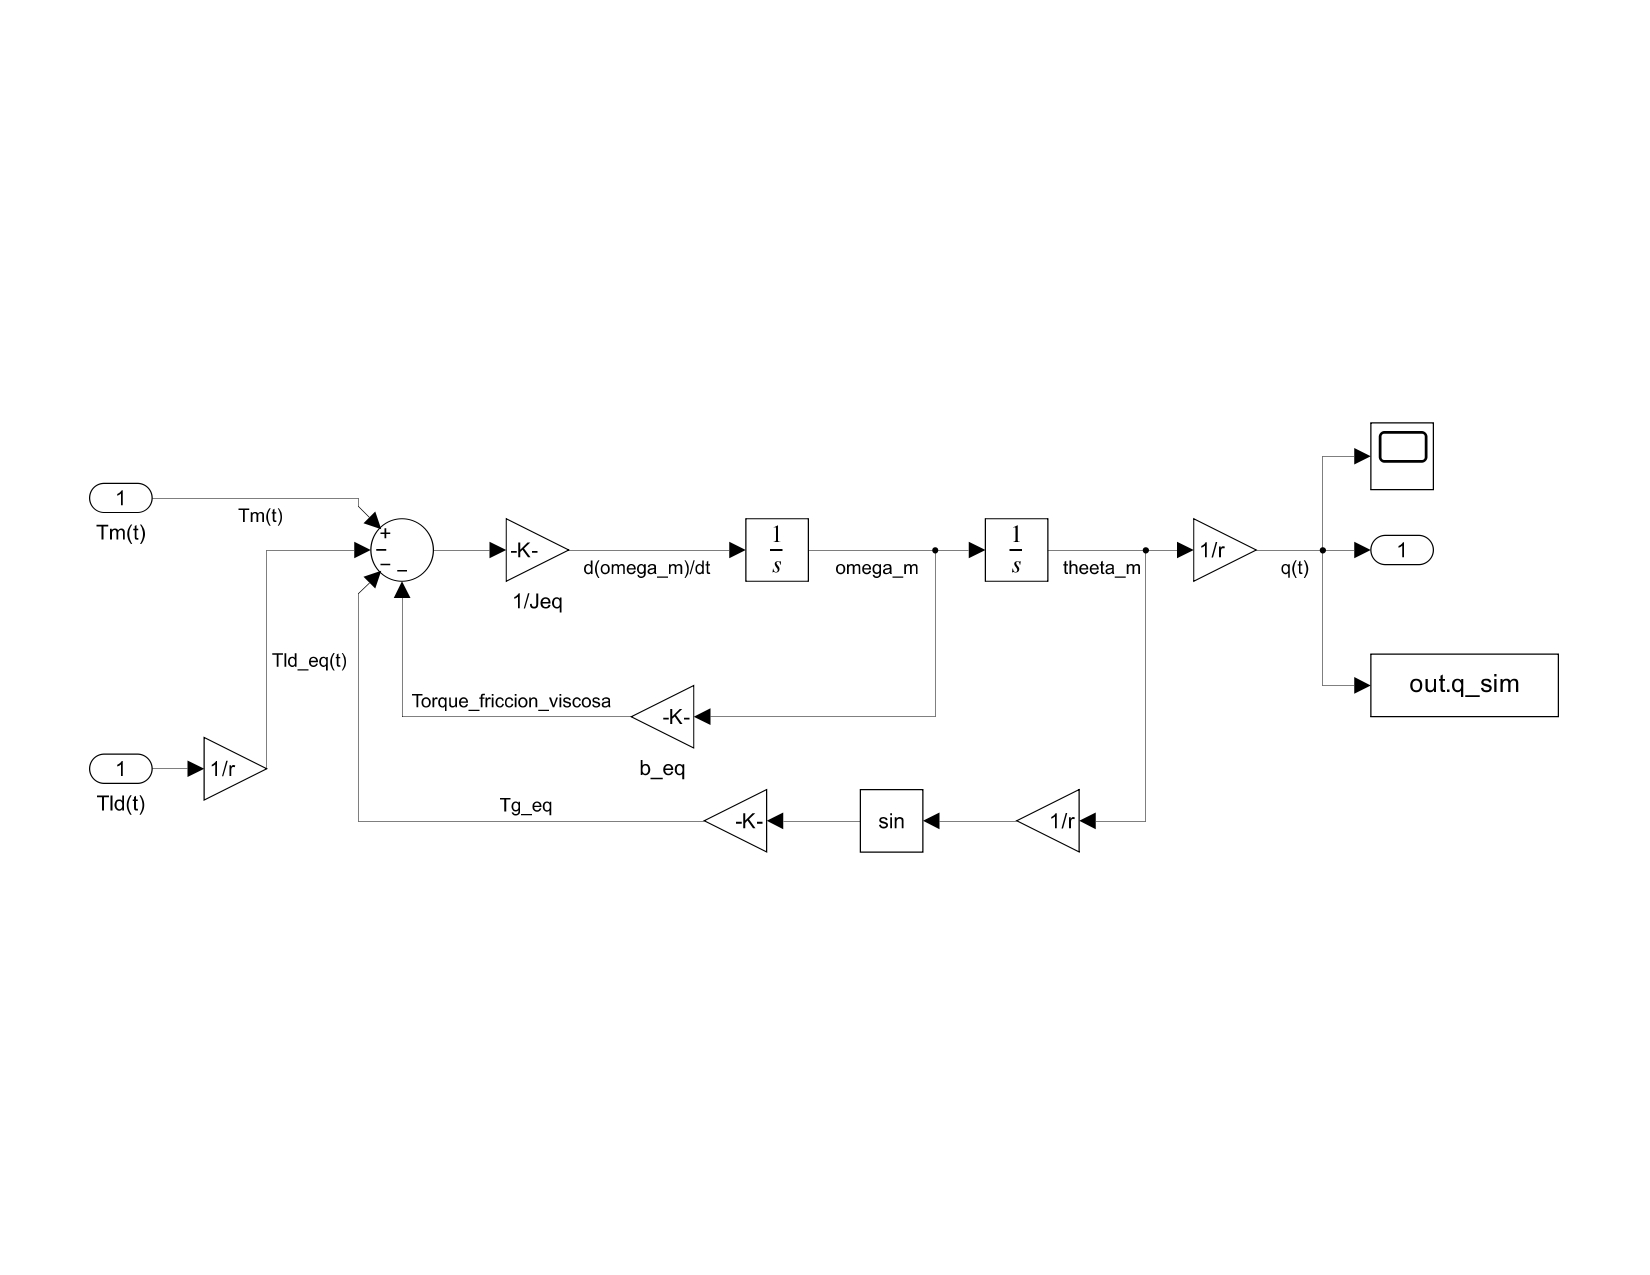
\includegraphics[width=0.95\textwidth]{subsistema_mecanico.jpg}
   	\caption{Diagrama de bloques del subsistema mecánico equivalente referido al eje del motor.}
   	\label{fig:diagrama_mecanico_equivalente}
   \end{figure}

El bloque equivalente tiene como entrada principal el torque electromagnético \(T_m(t)\), como perturbación el torque externo \(T_{ld}(t)\), y como salida mecánica de interés la posición articular \(q(t)\). La no linealidad del modelo aparece en el término gravitacional \(\sin(\theta_m/r)\).

\subsection{Síntesis parcial del punto 1}

A partir de las ecuaciones de la carga, la transmisión y el rotor del motor se obtuvo un modelo mecánico equivalente referido al eje del motor. El modelo conserva como estados principales la posición y velocidad del rotor, e incorpora la dinámica de la carga a través de parámetros equivalentes de inercia y fricción. Además, el torque gravitacional y la perturbación externa se reflejan al eje del motor mediante el factor \(1/r\). Este resultado permite utilizar el torque electromagnético \(T_m(t)\) como entrada mecánica directa del subsistema equivalente, lo cual será necesario para acoplar el modelo con las ecuaciones electromagnéticas de la PMSM.

% ---------------------------------------------------------
% SECCIONES PENDIENTES PARA COMPLETAR EL INFORME
% ---------------------------------------------------------

\subsection{Modelo dinámico global no lineal del sistema físico}

En esta sección se incorpora el subsistema electromagnético de la máquina PMSM y el subsistema térmico del bobinado de estator al modelo mecánico equivalente obtenido previamente. De esta manera, el torque electromagnético deja de considerarse una entrada externa genérica y pasa a calcularse a partir de las corrientes internas de la máquina en coordenadas de rotor. El modelo resultante es no lineal debido al acoplamiento electromecánico, a la dependencia de la resistencia con la temperatura, al producto entre corrientes en el torque de reluctancia, a los términos de fuerza contraelectromotriz y al torque gravitacional de la carga.

El modelo global se construye utilizando coordenadas electromagnéticas de rotor \(qd0\), obtenidas mediante la Transformación de Park. Para una variable trifásica genérica \(\mathbf{f}_{abcs}(t)=[f_{as}(t)\; f_{bs}(t)\; f_{cs}(t)]^T\), donde \(f\) puede representar tensión, corriente o flujo, la transformación directa adoptada es

\begin{equation}
    \begin{bmatrix}
        f_{qs}^{r}(t)\\
        f_{ds}^{r}(t)\\
        f_{0s}(t)
    \end{bmatrix}
    =
    \frac{2}{3}
    \begin{bmatrix}
        \cos\theta_r & \cos\left(\theta_r-\frac{2\pi}{3}\right) & \cos\left(\theta_r+\frac{2\pi}{3}\right)\\
        \sin\theta_r & \sin\left(\theta_r-\frac{2\pi}{3}\right) & \sin\left(\theta_r+\frac{2\pi}{3}\right)\\
        \frac{1}{2} & \frac{1}{2} & \frac{1}{2}
    \end{bmatrix}
    \begin{bmatrix}
        f_{as}(t)\\
        f_{bs}(t)\\
        f_{cs}(t)
    \end{bmatrix}.
    \label{eq:park_directa}
\end{equation}

La transformación inversa queda dada por

\begin{equation}
    \begin{bmatrix}
        f_{as}(t)\\
        f_{bs}(t)\\
        f_{cs}(t)
    \end{bmatrix}
    =
    \begin{bmatrix}
        \cos\theta_r & \sin\theta_r & 1\\
        \cos\left(\theta_r-\frac{2\pi}{3}\right) & \sin\left(\theta_r-\frac{2\pi}{3}\right) & 1\\
        \cos\left(\theta_r+\frac{2\pi}{3}\right) & \sin\left(\theta_r+\frac{2\pi}{3}\right) & 1
    \end{bmatrix}
    \begin{bmatrix}
        f_{qs}^{r}(t)\\
        f_{ds}^{r}(t)\\
        f_{0s}(t)
    \end{bmatrix}.
    \label{eq:park_inversa}
\end{equation}

Para el accionamiento considerado, el centro de estrella del estator es flotante y no accesible. Además, inicialmente se considera un sistema trifásico equilibrado. Por lo tanto, la componente homopolar no participa de la dinámica principal y se adopta

\begin{equation}
    i_{0s}(t) \equiv 0,
    \qquad
    v_{0s}(t) \equiv 0.
    \label{eq:homopolar_nula}
\end{equation}

\subsubsection{Variables de estado, entradas y salidas}

Se adopta como vector de estado global

\begin{equation}
    \mathbf{x}(t)=
    \begin{bmatrix}
        x_1(t)\\ x_2(t)\\ x_3(t)\\ x_4(t)\\ x_5(t)
    \end{bmatrix}
    =
    \begin{bmatrix}
        \theta_m(t)\\
        \omega_m(t)\\
        i_{qs}^{r}(t)\\
        i_{ds}^{r}(t)\\
        T_s^{\circ}(t)
    \end{bmatrix}.
    \label{eq:vector_estado_global_nl}
\end{equation}

Las entradas externas del modelo son

\begin{equation}
    \mathbf{u}(t)=
    \begin{bmatrix}
        u_1(t)\\ u_2(t)\\ u_3(t)\\ u_4(t)
    \end{bmatrix}
    =
    \begin{bmatrix}
        v_{qs}^{r}(t)\\
        v_{ds}^{r}(t)\\
        T_{ld}(t)\\
        T_{amb}^{\circ}(t)
    \end{bmatrix}.
    \label{eq:vector_entrada_global_nl}
\end{equation}

La salida principal de interés para el control de movimiento es la posición angular de la articulación:

\begin{equation}
    y(t)=q(t)=\theta_l(t)=\frac{\theta_m(t)}{r}=\frac{x_1(t)}{r}.
    \label{eq:salida_principal_q}
\end{equation}

Como salidas adicionales para análisis y realimentación pueden considerarse \(\theta_m(t)\), \(\omega_m(t)\), \(i_{qs}^{r}(t)\), \(i_{ds}^{r}(t)\), las corrientes reales de fase \(i_{as}(t), i_{bs}(t), i_{cs}(t)\) obtenidas mediante la Transformación de Park inversa, y la temperatura de estator \(T_s^{\circ}(t)\).

\subsubsection{Relaciones eléctricas rotor-estator}

La coordenada eléctrica del rotor se relaciona con la posición mecánica mediante

\begin{equation}
    \theta_r(t)=P_p\theta_m(t),
    \label{eq:theta_r}
\end{equation}

mientras que la velocidad eléctrica del rotor es

\begin{equation}
    \omega_r(t)=P_p\omega_m(t).
    \label{eq:omega_r}
\end{equation}

Para la máquina del proyecto se tiene \(P_p=3\) pares de polos. La resistencia de estator se modela dependiente de la temperatura del bobinado:

\begin{equation}
    R_s\left(T_s^{\circ}\right)
    =
    R_{sREF}
    \left[
    1+\alpha_{Cu}\left(T_s^{\circ}-T_{sREF}^{\circ}\right)
    \right].
    \label{eq:rs_temperatura}
\end{equation}

Con los valores nominales del proyecto:

\begin{equation}
    R_{sREF}=\SI{1.02}{\ohm},
    \qquad
    T_{sREF}^{\circ}=\SI{20}{\celsius},
    \qquad
    \alpha_{Cu}=3.9\times10^{-3}\ \si{\per\celsius}.
\end{equation}

\subsubsection{Modelo electromagnético de la PMSM en coordenadas \(qd\)}

Las ecuaciones de balance de tensión del estator, expresadas en coordenadas \(qd\) fijas al rotor, son

\begin{equation}
    v_{qs}^{r}(t)
    =
    R_s\left(T_s^{\circ}\right)i_{qs}^{r}(t)
    +
    L_q\frac{d i_{qs}^{r}(t)}{dt}
    +
    \left[\lambda_m^{\prime r}+L_d i_{ds}^{r}(t)\right]\omega_r(t),
    \label{eq:vq_pmsm}
\end{equation}

\begin{equation}
    v_{ds}^{r}(t)
    =
    R_s\left(T_s^{\circ}\right)i_{ds}^{r}(t)
    +
    L_d\frac{d i_{ds}^{r}(t)}{dt}
    -
    L_q i_{qs}^{r}(t)\omega_r(t).
    \label{eq:vd_pmsm}
\end{equation}

Despejando las derivadas de corriente, e incorporando \(\omega_r=P_p\omega_m\), se obtiene

\begin{equation}
    \frac{d i_{qs}^{r}}{dt}
    =
    \frac{
    v_{qs}^{r}
    -
    R_s\left(T_s^{\circ}\right)i_{qs}^{r}
    -
    \left(\lambda_m^{\prime r}+L_d i_{ds}^{r}\right)P_p\omega_m
    }{L_q},
    \label{eq:iq_dot_nl}
\end{equation}

\begin{equation}
    \frac{d i_{ds}^{r}}{dt}
    =
    \frac{
    v_{ds}^{r}
    -
    R_s\left(T_s^{\circ}\right)i_{ds}^{r}
    +
    L_q i_{qs}^{r}P_p\omega_m
    }{L_d}.
    \label{eq:id_dot_nl}
\end{equation}

El torque electromagnético generado por la PMSM está compuesto por un término debido a los imanes permanentes y un término de reluctancia:

\begin{equation}
    T_m(t)
    =
    \frac{3}{2}P_p\lambda_m^{\prime r}i_{qs}^{r}(t)
    +
    \frac{3}{2}P_p\left(L_d-L_q\right)i_{ds}^{r}(t)i_{qs}^{r}(t).
    \label{eq:torque_pmsm}
\end{equation}

Se definen las constantes

\begin{equation}
    K_t=\frac{3}{2}P_p\lambda_m^{\prime r},
    \qquad
    K_{rel}=\frac{3}{2}P_p\left(L_d-L_q\right),
    \label{eq:kt_krel}
\end{equation}

por lo que el torque puede escribirse como

\begin{equation}
    T_m(t)=K_t i_{qs}^{r}(t)+K_{rel}i_{ds}^{r}(t)i_{qs}^{r}(t).
    \label{eq:torque_pmsm_compacto}
\end{equation}

Con los parámetros nominales \(P_p=3\), \(\lambda_m^{\prime r}=\SI{0.016}{\weber}\), \(L_d=\SI{6.6e-3}{\henry}\) y \(L_q=\SI{5.8e-3}{\henry}\), se obtiene

\begin{equation}
    K_t=\SI{0.072}{\newton\meter\per\ampere},
    \qquad
    K_{rel}=\SI{0.0036}{\newton\meter\per\ampere\squared}.
    \label{eq:kt_krel_numerico}
\end{equation}

\subsubsection{Acoplamiento con el subsistema mecánico equivalente}

El modelo mecánico equivalente referido al eje del motor, desarrollado en el punto anterior, queda ahora acoplado al subsistema electromagnético mediante el torque \(T_m(t)\). Sustituyendo \eqref{eq:torque_pmsm_compacto} en \eqref{eq:modelo_mecanico_final}, se obtiene

\begin{equation}
    \dot{\omega}_m(t)
    =
    \frac{1}{J_{eq}}
    \left[
    K_t i_{qs}^{r}
    +
    K_{rel}i_{ds}^{r}i_{qs}^{r}
    -
    b_{eq}\omega_m
    -
    \frac{gk_l}{r}\sin\left(\frac{\theta_m}{r}\right)
    -
    \frac{T_{ld}}{r}
    \right].
    \label{eq:omega_dot_acoplada}
\end{equation}

El acoplamiento es bidireccional: la dinámica eléctrica genera el torque que acelera el eje mecánico, mientras que la velocidad mecánica determina la velocidad eléctrica \(\omega_r=P_p\omega_m\), la cual aparece en las ecuaciones de tensión de la máquina.

\subsubsection{Modelo térmico del estator}

Las pérdidas eléctricas por efecto Joule pueden calcularse en coordenadas \(qd0\). Considerando \(i_{0s}=0\), se tiene

\begin{equation}
    P_{s,perd}(t)
    =
    R_s\left(T_s^{\circ}\right)
    \frac{3}{2}
    \left[
    \left(i_{qs}^{r}(t)\right)^2+
    \left(i_{ds}^{r}(t)\right)^2
    \right].
    \label{eq:perdidas_joule_qd}
\end{equation}

El balance térmico simplificado del estator se expresa como

\begin{equation}
    P_{s,perd}(t)
    =
    C_{ts}\frac{dT_s^{\circ}(t)}{dt}
    +
    \frac{1}{R_{ts-amb}}
    \left[T_s^{\circ}(t)-T_{amb}^{\circ}(t)\right].
    \label{eq:balance_termico}
\end{equation}

Por lo tanto,

\begin{equation}
    \frac{dT_s^{\circ}}{dt}
    =
    \frac{1}{C_{ts}}
    \left[
    P_{s,perd}
    -
    \frac{T_s^{\circ}-T_{amb}^{\circ}}{R_{ts-amb}}
    \right].
    \label{eq:ts_dot}
\end{equation}

\subsubsection{Ecuaciones no lineales de estado}

Reuniendo las expresiones anteriores, el modelo dinámico global no lineal queda dado por

\begin{equation}
    \boxed{
    \begin{aligned}
        \dot{x}_1 &= x_2,\\[2mm]
        \dot{x}_2 &=
        \frac{1}{J_{eq}}
        \left[
        K_t x_3
        +
        K_{rel}x_4x_3
        -
        b_{eq}x_2
        -
        \frac{gk_l}{r}\sin\left(\frac{x_1}{r}\right)
        -
        \frac{u_3}{r}
        \right],\\[2mm]
        \dot{x}_3 &=
        \frac{
        u_1
        -
        R_s(x_5)x_3
        -
        \left(\lambda_m^{\prime r}+L_d x_4\right)P_p x_2
        }{L_q},\\[2mm]
        \dot{x}_4 &=
        \frac{
        u_2
        -
        R_s(x_5)x_4
        +
        L_q x_3 P_p x_2
        }{L_d},\\[2mm]
        \dot{x}_5 &=
        \frac{1}{C_{ts}}
        \left[
        R_s(x_5)\frac{3}{2}\left(x_3^2+x_4^2\right)
        -
        \frac{x_5-u_4}{R_{ts-amb}}
        \right].
    \end{aligned}
    }
    \label{eq:modelo_global_nl}
\end{equation}

La salida principal es

\begin{equation}
    y(t)=q(t)=\frac{x_1(t)}{r}.
    \label{eq:salida_global_nl}
\end{equation}

El estado inicial genérico se define como

\begin{equation}
    \mathbf{x}(t_0)=
    \begin{bmatrix}
        \theta_m(t_0) & \omega_m(t_0) & i_{qs}^{r}(t_0) & i_{ds}^{r}(t_0) & T_s^{\circ}(t_0)
    \end{bmatrix}^{T}.
    \label{eq:estado_inicial_generico}
\end{equation}

Para las simulaciones iniciales del sistema detenido en equilibrio se adoptará

\begin{equation}
    \theta_m(t_0)=0,
    \qquad
    \omega_m(t_0)=0,
    \qquad
    i_{qs}^{r}(t_0)=0,
    \qquad
    i_{ds}^{r}(t_0)=0,
    \qquad
    T_s^{\circ}(t_0)=T_{amb}^{\circ}(t_0)=\SI{40}{\celsius}.
    \label{eq:estado_inicial_equilibrio}
\end{equation}

\subsubsection{Parámetros eléctricos y térmicos nominales}

En la Tabla \ref{tab:parametros_electricos_termicos} se resumen los parámetros eléctricos y térmicos utilizados para el modelo global.

\begin{table}[H]
    \centering
    \caption{Parámetros eléctricos y térmicos nominales de la PMSM.}
    \label{tab:parametros_electricos_termicos}
    \begin{tabular}{lll}
        \toprule
        Parámetro & Descripción & Valor nominal \\
        \midrule
        \(P_p\) & Pares de polos magnéticos & \(3\) \\
        \(\lambda_m^{\prime r}\) & Flujo de imanes concatenado & \(\SI{0.016}{\weber}\) \\
        \(L_q\) & Inductancia eje \(q\) & \(\SI{5.8e-3}{\henry}\) \\
        \(L_d\) & Inductancia eje \(d\) & \(\SI{6.6e-3}{\henry}\) \\
        \(L_{ls}\) & Inductancia de dispersión & \(\SI{0.8e-3}{\henry}\) \\
        \(R_{sREF}\) & Resistencia de estator a \(\SI{20}{\celsius}\) & \(\SI{1.02}{\ohm}\) \\
        \(\alpha_{Cu}\) & Coeficiente térmico del cobre & \(3.9\times10^{-3}\ \si{\per\celsius}\) \\
        \(C_{ts}\) & Capacitancia térmica del estator & \(\SI{0.818}{\watt\per\celsius\per\second}\) \\
        \(R_{ts-amb}\) & Resistencia térmica estator-ambiente & \(\SI{146.7}{\celsius\per\watt}\) \\
        \bottomrule
    \end{tabular}
\end{table}

\subsection{Linealización Jacobiana y modelo LPV}

El modelo no lineal obtenido en \eqref{eq:modelo_global_nl} puede linealizarse localmente alrededor de un punto genérico de operación. Se define el punto de operación

\begin{equation}
    \mathbf{x}^{o}=
    \begin{bmatrix}
        \theta_m^{o}\\
        \omega_m^{o}\\
        I_q^{o}\\
        I_d^{o}\\
        T_s^{o}
    \end{bmatrix},
    \qquad
    \mathbf{u}^{o}=
    \begin{bmatrix}
        V_q^{o}\\
        V_d^{o}\\
        T_{ld}^{o}\\
        T_{amb}^{o}
    \end{bmatrix}.
    \label{eq:punto_operacion_generico}
\end{equation}

El modelo linealizado en pequeñas variaciones queda expresado como

\begin{equation}
    \Delta \dot{\mathbf{x}}(t)
    =
    A\left(\mathbf{x}^{o},\mathbf{u}^{o}\right)\Delta\mathbf{x}(t)
    +
    B\left(\mathbf{x}^{o},\mathbf{u}^{o}\right)\Delta\mathbf{u}(t),
    \label{eq:modelo_lpv}
\end{equation}

\begin{equation}
    \Delta \mathbf{y}(t)
    =
    C\Delta\mathbf{x}(t)+D\Delta\mathbf{u}(t),
    \label{eq:salida_lpv}
\end{equation}

con

\begin{equation}
    A=\left.\frac{\partial \mathbf{f}}{\partial \mathbf{x}}\right|_{\mathbf{x}^{o},\mathbf{u}^{o}},
    \qquad
    B=\left.\frac{\partial \mathbf{f}}{\partial \mathbf{u}}\right|_{\mathbf{x}^{o},\mathbf{u}^{o}}.
    \label{eq:jacobianos}
\end{equation}

Para abreviar, se define

\begin{equation}
    R_s^{o}=R_s(T_s^{o}),
    \qquad
    R_T=\frac{dR_s}{dT_s}=R_{sREF}\alpha_{Cu}.
    \label{eq:rs_rt_lpv}
\end{equation}

La matriz jacobiana de estado queda

\begin{equation}
\small
    A=
    \begin{bmatrix}
        0 & 1 & 0 & 0 & 0\\[1mm]
        -\dfrac{gk_l}{J_{eq}r^2}\cos\left(\dfrac{\theta_m^{o}}{r}\right)
        & -\dfrac{b_{eq}}{J_{eq}}
        & \dfrac{K_t+K_{rel}I_d^{o}}{J_{eq}}
        & \dfrac{K_{rel}I_q^{o}}{J_{eq}}
        & 0\\[4mm]
        0
        & -\dfrac{P_p\left(\lambda_m^{\prime r}+L_dI_d^{o}\right)}{L_q}
        & -\dfrac{R_s^{o}}{L_q}
        & -\dfrac{L_dP_p\omega_m^{o}}{L_q}
        & -\dfrac{R_T I_q^{o}}{L_q}\\[4mm]
        0
        & \dfrac{L_qP_pI_q^{o}}{L_d}
        & \dfrac{L_qP_p\omega_m^{o}}{L_d}
        & -\dfrac{R_s^{o}}{L_d}
        & -\dfrac{R_T I_d^{o}}{L_d}\\[4mm]
        0
        & 0
        & \dfrac{3R_s^{o}I_q^{o}}{C_{ts}}
        & \dfrac{3R_s^{o}I_d^{o}}{C_{ts}}
        & \dfrac{\frac{3}{2}R_T\left[(I_q^{o})^2+(I_d^{o})^2\right]-\frac{1}{R_{ts-amb}}}{C_{ts}}
    \end{bmatrix}.
    \label{eq:matriz_a_lpv}
\end{equation}

La matriz de entrada, considerando \(\Delta\mathbf{u}=[\Delta v_q\;\Delta v_d\;\Delta T_{ld}\;\Delta T_{amb}^{\circ}]^T\), es

\begin{equation}
    B=
    \begin{bmatrix}
        0 & 0 & 0 & 0\\[1mm]
        0 & 0 & -\dfrac{1}{J_{eq}r} & 0\\[4mm]
        \dfrac{1}{L_q} & 0 & 0 & 0\\[4mm]
        0 & \dfrac{1}{L_d} & 0 & 0\\[4mm]
        0 & 0 & 0 & \dfrac{1}{R_{ts-amb}C_{ts}}
    \end{bmatrix}.
    \label{eq:matriz_b_lpv}
\end{equation}

Para la salida principal \(q(t)=\theta_m(t)/r\), se tiene

\begin{equation}
    C_q=
    \begin{bmatrix}
        \frac{1}{r} & 0 & 0 & 0 & 0
    \end{bmatrix},
    \qquad
    D_q=
    \begin{bmatrix}
        0 & 0 & 0 & 0
    \end{bmatrix}.
    \label{eq:c_d_q_lpv}
\end{equation}

Este modelo se denomina LPV porque las matrices dependen del punto de operación. En particular, aparecen como parámetros variables \(\theta_m^{o}\), \(\omega_m^{o}\), \(I_q^{o}\), \(I_d^{o}\) y \(T_s^{o}\). Por lo tanto, el comportamiento local del sistema cambia cuando se modifica la velocidad, la carga, las corrientes de operación o la temperatura del bobinado.

\subsection{Linealización por retroalimentación y modelo LTI equivalente}

La estrategia de control vectorial con campo orientado impone la condición

\begin{equation}
    i_{ds}^{r}(t)\equiv 0.
    \label{eq:id_cero}
\end{equation}

Con esta condición, el eje \(d\) queda asociado al flujo y el eje \(q\) queda asociado principalmente a la producción de torque. En consecuencia, el torque electromagnético se reduce a

\begin{equation}
    T_m(t)=K_t i_{qs}^{r}(t),
    \label{eq:torque_id_cero}
\end{equation}

ya que el término de reluctancia desaparece.

\subsubsection{Ley mínima de desacoplamiento en eje \(d\)}

La dinámica del eje \(d\) está dada por

\begin{equation}
    \dot{i}_{ds}^{r}
    =
    \frac{
    v_{ds}^{r}
    -
    R_s i_{ds}^{r}
    +
    L_q i_{qs}^{r}\omega_r
    }{L_d}.
    \label{eq:dinamica_d_desacople}
\end{equation}

Para imponer \(i_{ds}^{r}(t)=0\) en forma invariante se requiere también \(\dot{i}_{ds}^{r}(t)=0\). Si \(i_{ds}^{r}=0\), resulta

\begin{equation}
    0=
    \frac{
    v_{ds}^{r}
    +
    L_q i_{qs}^{r}\omega_r
    }{L_d}.
\end{equation}

Por lo tanto, la ley mínima de control no lineal en eje \(d\) es

\begin{equation}
    \boxed{
    v_{ds}^{r*}(t)
    =
    -L_q i_{qs}^{r}(t)\omega_r(t)
    =
    -L_q i_{qs}^{r}(t)P_p\omega_m(t)
    }.
    \label{eq:ley_desacople_d}
\end{equation}

Esta ley permite cumplir \(i_{ds}^{r}(t)\equiv0\) siempre que se verifique la hipótesis de estado inicial

\begin{equation}
    i_{ds}^{r}(t_0)=0.
    \label{eq:hipotesis_id0}
\end{equation}

\subsubsection{Dinámica residual en eje \(d\)}

Si se aplica la ley \eqref{eq:ley_desacople_d}, pero el estado inicial no cumple \(i_{ds}^{r}(t_0)=0\), la dinámica residual del eje \(d\) queda

\begin{equation}
    \dot{i}_{ds}^{r}(t)
    =
    -\frac{R_s}{L_d}i_{ds}^{r}(t).
    \label{eq:dinamica_residual_id}
\end{equation}

Por lo tanto,

\begin{equation}
    i_{ds}^{r}(t)
    =
    i_{ds}^{r}(t_0)e^{-\frac{R_s}{L_d}(t-t_0)}.
    \label{eq:solucion_residual_id}
\end{equation}

Con \(R_s=\SI{1.02}{\ohm}\) y \(L_d=\SI{6.6e-3}{\henry}\), la constante de tiempo eléctrica residual es

\begin{equation}
    \tau_d=\frac{L_d}{R_s}=\frac{6.6\times10^{-3}}{1.02}\approx\SI{6.47}{\milli\second}.
    \label{eq:tau_d_residual}
\end{equation}

Esto implica que un error inicial en \(i_d\) desaparece mucho más rápido que la dinámica mecánica. El acoplamiento residual no lineal asociado aparece en el torque de reluctancia \(K_{rel}i_d i_q\). Dicho término puede despreciarse en régimen forzado cuando \(i_d\) decae hacia cero y cuando \(K_{rel}\) es pequeño frente al término principal \(K_t i_q\).

\subsubsection{Ley complementaria de desacoplamiento en eje \(q\)}

La dinámica del eje \(q\) incluye el término de fuerza contraelectromotriz

\begin{equation}
    \left(\lambda_m^{\prime r}+L_d i_{ds}^{r}\right)\omega_r.
\end{equation}

Para eliminar este acoplamiento, se define una nueva entrada auxiliar \(u_q(t)\) tal que

\begin{equation}
    \boxed{
    v_{qs}^{r}(t)
    =
    u_q(t)
    +
    \left(\lambda_m^{\prime r}+L_d i_{ds}^{r}(t)\right)\omega_r(t)
    }.
    \label{eq:ley_desacople_q}
\end{equation}

Sustituyendo \eqref{eq:ley_desacople_q} en la dinámica de \(i_q\), se obtiene

\begin{equation}
    \dot{i}_{qs}^{r}(t)
    =
    -\frac{R_s}{L_q}i_{qs}^{r}(t)
    +
    \frac{1}{L_q}u_q(t).
    \label{eq:iq_desacoplada}
\end{equation}

Si además se cumple \(i_{ds}^{r}(t)=0\), el sistema eléctrico queda desacoplado y lineal en el eje \(q\).

\subsubsection{Modelo LTI equivalente aumentado}

Para obtener un modelo LTI equivalente se considera la dinámica alrededor del equilibrio mecánico \(\theta_m=0\). En ese entorno,

\begin{equation}
    \sin\left(\frac{\theta_m}{r}\right)
    \approx
    \frac{\theta_m}{r}.
    \label{eq:aprox_seno}
\end{equation}

Entonces el torque gravitacional equivalente puede aproximarse como

\begin{equation}
    \frac{gk_l}{r}\sin\left(\frac{\theta_m}{r}\right)
    \approx
    \frac{gk_l}{r^2}\theta_m.
    \label{eq:torque_gravitacional_lti}
\end{equation}

El modelo LTI equivalente aumentado queda

\begin{equation}
    \dot{\theta}_m=\omega_m,
    \label{eq:lti_theta_dot}
\end{equation}

\begin{equation}
    \dot{\omega}_m
    =
    -\frac{gk_l}{J_{eq}r^2}\theta_m
    -
    \frac{b_{eq}}{J_{eq}}\omega_m
    +
    \frac{K_t}{J_{eq}}i_q
    -
    \frac{1}{J_{eq}r}T_{ld},
    \label{eq:lti_omega_dot}
\end{equation}

\begin{equation}
    \dot{i}_q
    =
    -\frac{R_s}{L_q}i_q
    +
    \frac{1}{L_q}u_q,
    \label{eq:lti_iq_dot}
\end{equation}

\begin{equation}
    \dot{i}_d
    =
    -\frac{R_s}{L_d}i_d.
    \label{eq:lti_id_dot}
\end{equation}

Para conservar la dinámica térmica como modo lineal independiente, se toma la potencia de pérdidas \(P_{s,perd}\) como entrada auxiliar:

\begin{equation}
    \dot{T}_s^{\circ}
    =
    -\frac{1}{R_{ts-amb}C_{ts}}T_s^{\circ}
    +
    \frac{1}{C_{ts}}P_{s,perd}
    +
    \frac{1}{R_{ts-amb}C_{ts}}T_{amb}^{\circ}.
    \label{eq:lti_ts_dot}
\end{equation}

Tomando

\begin{equation}
    \mathbf{x}_{LTI}=\begin{bmatrix}\theta_m & \omega_m & i_q & i_d & T_s^{\circ}\end{bmatrix}^{T},
    \qquad
    \mathbf{u}_{LTI}=\begin{bmatrix}u_q & T_{ld} & P_{s,perd} & T_{amb}^{\circ}\end{bmatrix}^{T},
    \label{eq:x_u_lti}
\end{equation}

se obtiene

\begin{equation}
    \dot{\mathbf{x}}_{LTI}=A_{LTI}\mathbf{x}_{LTI}+B_{LTI}\mathbf{u}_{LTI},
    \label{eq:ss_lti}
\end{equation}

con

\begin{equation}
    A_{LTI}=
    \begin{bmatrix}
        0 & 1 & 0 & 0 & 0\\[1mm]
        -\dfrac{gk_l}{J_{eq}r^2} & -\dfrac{b_{eq}}{J_{eq}} & \dfrac{K_t}{J_{eq}} & 0 & 0\\[4mm]
        0 & 0 & -\dfrac{R_s}{L_q} & 0 & 0\\[4mm]
        0 & 0 & 0 & -\dfrac{R_s}{L_d} & 0\\[4mm]
        0 & 0 & 0 & 0 & -\dfrac{1}{R_{ts-amb}C_{ts}}
    \end{bmatrix},
    \label{eq:a_lti_simbolica}
\end{equation}

\begin{equation}
    B_{LTI}=
    \begin{bmatrix}
        0 & 0 & 0 & 0\\[1mm]
        0 & -\dfrac{1}{J_{eq}r} & 0 & 0\\[4mm]
        \dfrac{1}{L_q} & 0 & 0 & 0\\[4mm]
        0 & 0 & 0 & 0\\[4mm]
        0 & 0 & \dfrac{1}{C_{ts}} & \dfrac{1}{R_{ts-amb}C_{ts}}
    \end{bmatrix}.
    \label{eq:b_lti_simbolica}
\end{equation}

Para la salida articular,

\begin{equation}
    C_q=\begin{bmatrix}\dfrac{1}{r} & 0 & 0 & 0 & 0\end{bmatrix},
    \qquad
    D_q=\begin{bmatrix}0 & 0 & 0 & 0\end{bmatrix}.
    \label{eq:cq_lti}
\end{equation}

\subsubsection{Matrices LTI nominales}

Utilizando los valores nominales sin carga útil y \(R_s=R_{sREF}=\SI{1.02}{\ohm}\), se obtienen los siguientes coeficientes:

\begin{equation}
    \frac{gk_l}{J_{eq}r^2}=8.605,
    \qquad
    \frac{b_{eq}}{J_{eq}}=1.109,
    \qquad
    \frac{K_t}{J_{eq}}=3639.172,
\end{equation}

\begin{equation}
    \frac{R_s}{L_q}=175.862,
    \qquad
    \frac{R_s}{L_d}=154.545,
    \qquad
    \frac{1}{R_{ts-amb}C_{ts}}=0.00833.
\end{equation}

Por lo tanto,

\begin{equation}
    A_{LTI}\approx
    \begin{bmatrix}
        0 & 1 & 0 & 0 & 0\\
        -8.605 & -1.109 & 3639.172 & 0 & 0\\
        0 & 0 & -175.862 & 0 & 0\\
        0 & 0 & 0 & -154.545 & 0\\
        0 & 0 & 0 & 0 & -0.00833
    \end{bmatrix},
    \label{eq:a_lti_numerica}
\end{equation}

\begin{equation}
    B_{LTI}\approx
    \begin{bmatrix}
        0 & 0 & 0 & 0\\
        0 & -421.200 & 0 & 0\\
        172.414 & 0 & 0 & 0\\
        0 & 0 & 0 & 0\\
        0 & 0 & 1.222 & 0.00833
    \end{bmatrix}.
    \label{eq:b_lti_numerica}
\end{equation}

\subsubsection{Funciones de transferencia hacia \(\theta_m(t)\)}

A partir del modelo LTI equivalente aumentado se pueden obtener las funciones de transferencia desde la entrada auxiliar de tensión \(u_q(t)\) y desde la perturbación \(T_{ld}(t)\) hacia la posición del eje del motor \(\theta_m(t)\). Se considera estado inicial nulo para la obtención de funciones de transferencia.

Desde \(u_q(t)\) hasta \(\theta_m(t)\):

\begin{equation}
    \frac{\Theta_m(s)}{U_q(s)}
    =
    \frac{
    \dfrac{K_t}{J_{eq}}\dfrac{1}{L_q}
    }{
    \left(s+\dfrac{R_s}{L_q}\right)
    \left(
    s^2+\dfrac{b_{eq}}{J_{eq}}s+\dfrac{gk_l}{J_{eq}r^2}
    \right)
    }.
    \label{eq:ft_theta_uq_simbolica}
\end{equation}

Numéricamente,

\begin{equation}
    \frac{\Theta_m(s)}{U_q(s)}
    \approx
    \frac{6.2744\times10^{5}}{s^3+176.971s^2+203.665s+1513.354}.
    \label{eq:ft_theta_uq_numerica}
\end{equation}

Desde la perturbación \(T_{ld}(t)\) hasta \(\theta_m(t)\):

\begin{equation}
    \frac{\Theta_m(s)}{T_{ld}(s)}
    =
    \frac{
    -\dfrac{1}{J_{eq}r}
    }{
    s^2+\dfrac{b_{eq}}{J_{eq}}s+\dfrac{gk_l}{J_{eq}r^2}
    }.
    \label{eq:ft_theta_tld_simbolica}
\end{equation}

Numéricamente,

\begin{equation}
    \frac{\Theta_m(s)}{T_{ld}(s)}
    \approx
    \frac{-421.200}{s^2+1.109s+8.605}.
    \label{eq:ft_theta_tld_numerica}
\end{equation}

Los estados \(i_d\) y \(T_s^{\circ}\) no aparecen en las funciones de transferencia anteriores hacia \(\theta_m\) porque, bajo la linealización por retroalimentación propuesta, quedan desacoplados de la dinámica mecánica dominante. El estado \(i_d\) queda como modo eléctrico residual y la temperatura queda como una dinámica térmica lenta excitada por la potencia de pérdidas.

\subsection{Análisis a lazo abierto}
\textit{Sección pendiente. Aquí se analizarán polos, ceros, estabilidad, controlabilidad, observabilidad y respuestas temporales del sistema físico sin controlador externo de movimiento.}

\subsection{Diseño del sistema de control}
\textit{Sección pendiente. Aquí se desarrollarán el modulador de torque, los lazos de corriente, el observador de estado y el controlador externo de movimiento.}

\subsection{Simulación, resultados y verificación de restricciones}
\textit{Sección pendiente. Aquí se presentarán las simulaciones del sistema completo, el seguimiento de referencia, el rechazo de perturbaciones y la verificación de límites de corriente, tensión, velocidad, torque y temperatura.}

% ---------------------------------------------------------
% CONCLUSIONES
% ---------------------------------------------------------
\section{Conclusiones}

Hasta esta etapa se obtuvo el modelo mecánico equivalente referido al eje del motor y se incorporaron los subsistemas electromagnético y térmico de la PMSM. El modelo global no lineal permite representar el acoplamiento entre tensiones, corrientes, torque electromagnético, movimiento mecánico y temperatura del estator. Además, se obtuvo un modelo LPV mediante linealización Jacobiana y un modelo LTI equivalente aumentado aplicando una estrategia de campo orientado con \(i_{ds}^{r}(t)\equiv0\) y leyes de desacoplamiento en los ejes \(d\) y \(q\). Este modelo LTI será utilizado como base para el análisis a lazo abierto y el posterior diseño de control.

\textit{Nota: esta sección debe actualizarse al finalizar el proyecto completo, incorporando conclusiones sobre control, observador, discretización y resultados de simulación.}

% ---------------------------------------------------------
% REFERENCIAS
% ---------------------------------------------------------
\begin{thebibliography}{9}

\bibitem{guia_trabajo}
G. L. Julián, \textit{Proyecto Global Integrador: Guía de Trabajo y Especificaciones}, Espacio Curricular: Automática y Máquinas Eléctricas, Facultad de Ingeniería, Universidad Nacional de Cuyo, Rev. 0, 2026.

\bibitem{guia_informe}
G. L. Julián, \textit{Proyecto Global Integrador: Guía para preparar Informe Técnico}, Espacio Curricular: Automática y Máquinas Eléctricas, Facultad de Ingeniería, Universidad Nacional de Cuyo, Rev. 0, 2025.

\bibitem{krause}
P. C. Krause, O. Wasynczuk, S. D. Sudhoff y S. Pekarek, \textit{Analysis of Electric Machinery and Drive Systems}, 3rd ed. Hoboken, NJ, USA: Wiley-IEEE Press, 2013.

\bibitem{astrom}
K. J. Åström y R. M. Murray, \textit{Feedback Systems: An Introduction for Scientists and Engineers}. Princeton, NJ, USA: Princeton University Press, 2008.

\end{thebibliography}

\end{document}
